\documentclass[mathserif]{beamer} 
\usepackage{eulervm} %красивый математический шрифт - по желанию
\usepackage{ulem} %зачёркивания
\usepackage{bm} %особо жирный математический
\usepackage{schemata} %для красивых блочных переходов, пользуюсь редко
\usepackage{mathtools} %улучшенная работа с типографией в math mode
\setbeamertemplate{navigation symbols}{} %отключает управляющие символы в правом нижнем углу
\usefonttheme{professionalfonts}
\usepackage{cmap} %чтобы были работающие гиперссылки
\usepackage{makeidx,fancybox,tikz}
\usetikzlibrary{automata, positioning, arrows,patterns}
\usetikzlibrary{arrows.meta}
\usepackage{tempora} %по желанию -- русские штрифты с засечками

\mode<presentation>
{
  \usetheme{CambridgeUS} 
  \usecolortheme{dove} 
}
\usepackage[T1,T2A]{fontenc}
\usepackage[utf8]{inputenc}
\usepackage[english,russian]{babel}
\usepackage{amsmath,mathrsfs} %ещё больше математических символов
\usepackage{amstext}
\usepackage{graphicx,relsize}
\graphicspath{ {./../images/} }

\usepackage{color}
\definecolor{gray}{rgb}{0.4,.4,0.4} %здесь можно определить собственные цвета
\definecolor{grey80}{rgb}{0.8,.8,0.8}
\definecolor{grey90}{rgb}{0.9,.9,0.9}
\definecolor{grey95}{rgb}{0.95,.95,0.95}
\newcommand\redstroke{\bgroup\markoverwith
{\textcolor{red}{\rule[0.5ex]{2pt}{1.5pt}}}\ULon} %зачёркивание жирной красной чертой

\newcommand\reduline{\bgroup\markoverwith
{\textcolor{red}{\rule[-0.5ex]{2pt}{1.5pt}}}\ULon}%подчёркивание жирной красной чертой

\newcommand\bluline{\bgroup\markoverwith
{\textcolor{blue}{\rule[-0.5ex]{2pt}{1.5pt}}}\ULon}

\newcommand\bolduline{\bgroup\markoverwith
{\textcolor{white}{\rule[-0.5ex]{2pt}{1.5pt}}}\ULon}

\title[] {Автомат Томпсона}

\author[Chipollino]{Лучшая команда разработчиков по ТФЯ} % :))
\date[] 
{2022 г.}
\subject{Computer Science}

\newcommand{\Lang}{\mathscr{L}} %макрос для языка регулярки или автомата
\def\logor{\mathrel{\vee}} %отрендеренные логические операторы (с правильными интервалами)
\def\logimpl{\mathrel{\Rightarrow}}
\def\Linearize{\mathtt{Linearize}} %названия операций интерпретатора записываем моноширинным
\def\First{\mathrm{First}} %названия прочих операций записываем обычным шрифтом, но не тем, который в math mode по умолчанию
\def\Last{\mathrm{Last}}
\def\Follow{\mathrm{Follow}}
\def\Glushkov{\mathtt{Glushkov}}
\def\Thompson{\mathtt{Thompson}}
\def\logand{\mathrel{\&}}
\def\lognot{\mathop{\neg}}
\def\iff{\mathrel{\Leftrightarrow}}
\def\quantall#1{\mathop{\forall #1}}
\def\quantex#1{\mathop{\exists #1}} 
\def\alter{\ensuremath{\mathrel{\vert}}}%отрендеренные регулярные операторы 
\def\star{\ensuremath{^{*}}}%отрендеренные регулярные операторы 
\def\regexpstr#1{\mathtt{#1}}%буквы внутри регулярок переписываются в моноширинный
\newcommand{\Nat}{\mathbb N}
\newcommand{\empt}{\varepsilon} %пустое слово
\newcommand{\bottom}{\bot} %противоречие
\newcommand{\rar}{\rightarrow} %стрелка вправо. Для экономии букв.
\newcommand{\RegExp}{\mathcal{RE}} %макрос для обозначения множества всех регулярок
\def\Aut{\mathscr{A}}
\newcommand{\seq}{\;{=}\;}
\newenvironment{wideitemize}{\itemize\addtolength{\itemsep}{8pt}}{\enditemize}
\newcommand{\transit}[1]{\overset{#1}{\longrightarrow}}
%в преамбулу можно и нужно добавлять свои макросы

\begin{document}

\maketitle
\section{Основные понятия}
% overall documentation : frame 
\begin{frame}{Адгоритм Томпсона и НКА}
    \vspace{-5pt}
    \begin{block}{\bf Основные сведения}
        В информатике алгоритм построения Томпсона представляет собой метод преобразования регулярного выражения в эквивалентный недетерминированный конечный автомат (НКА). Этот НКА можно использовать для сопоставления строк с регулярным выражением.
        Регулярные выражения и недетерминированные конечные автоматы - это два представления формальных языков.
    \end{block}
\end{frame}% overall documentation

% descriptive documentation : frame 
\begin{frame}{Недетерминированные КА}\only<3> {\vspace{-5pt}}
    \vspace{-5pt}
    \only<1> {
        \begin{block}{\bf Определение}
            Недетерминированный конечный автомат (НКА) -- это детерминированный конечный автомат (ДКА), который не выполняет следующие условия:
            \begin{itemize}
                \item любой его переход единственным образом определяется по текущему состоянию и входному символу;
                \item чтение входного символа требуется для каждого изменения состояния.
            \end{itemize}
        \end{block}
    }
    \only<2> {
        \begin{block}{Определение}
            Недетерминированный конечный автомат (NFA) --- это пятёрка $\Aut\seq\langle Q,\Sigma, q_0, F, \delta \rangle${, где:
                    \begin{itemize}
                        \item $Q$ --- множество состояний;
                        \item $\Sigma$ --- алфавит терминалов;
                        \item $\delta$ --- множество правил перехода вида $\langle q_i, (a_i|\empt), M_i\rangle$, где $q_i\in Q$, $a_i\in \Sigma$, $M_i\in 2^Q$;
                        \item $q_0\in Q$ --- начальное состояние;
                        \item $F\subseteq Q$ --- множество конечных состояний.
                    \end{itemize}}
        \end{block}

        Сокращаем: $\langle q_1, a, q_2\rangle\in \delta\iff \langle q_1,a,M\rangle\in\delta\logand q_2\in M$.
    }
    \only<3> {
        \begin{wideitemize}
            \item $q \overset{\empt}{\longrightarrow} q'\iff (q=q')\logor\exists p_1,\dots,p_{k}(\langle q,\empt, p_1\rangle\in \delta\logand \langle p_k,\empt,q'\rangle\in\delta\logand\forall i,1\leq i<k\langle p_i,\empt,p_{i+1}\rangle\in\delta)$.

            \item $q\overset{a}{\longrightarrow}q'\iff \exists p,p'(q\overset{\empt}{\longrightarrow}p\logand \langle p, a, p'\rangle\in\delta\logand p'\overset{\empt}{\longrightarrow}q')$.

            \item $q \overset{a_1\dots a_k}{\longrightarrow} q'\iff \exists p_1,\dots,p_{k-1}(q\overset{a_1}{\longrightarrow}p_1\logand p_{k-1}\overset{a_k}{\longrightarrow}q'\logand \forall i,1\leq i<k-1(p_i\overset{a_{i+1}}{\longrightarrow}p_{i+1}))$.
        \end{wideitemize}

        \vspace{-5pt}
        \begin{block}{Определение}
            Язык $\Lang$, распознаваемый НКА $\Aut$ --- это множество слов $\bigl\lbrace{}w\mid\exists q\in F (q_0\transit{w}q)\bigr\rbrace{}$.
        \end{block}
    }
\end{frame} % descriptive documentation

\begin{frame}{Пример НКА}
    \vspace{-5pt}
    \begin{center}
        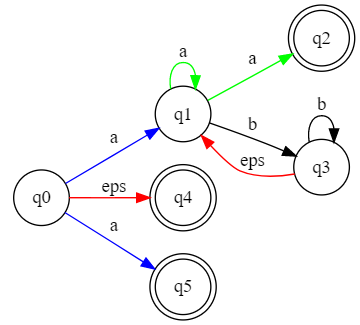
\includegraphics[width=3in, keepaspectratio]{tompson1.png} % the NFA example diagram placeholder
    \end{center}
\end{frame}% descriptive documentation

\section{Автомат Томпсона}
% descriptive documentation : frame
\begin{frame}{Конструкция автомата Томпсона}\only<2> {\vspace{-5pt}}
    \vspace{-5pt}
    \begin{block}{\bf Алгоритм построения $\Thompson(r)$}
        \only<1-2>{Алгоритм работает рекурсивно, разбивая выражение на составляющие его подвыражения, из которых будет построен НКА с использованием набора правил. Точнее, из регулярного выражения $r$ полученный автомат $A$ с переходной функцией $\delta$ учитывает следующие свойства:}
        \begin{wideitemize}
            \only<1> {
                \item $A$ имеет ровно одно начальное состояние $q_{0}$, которое недоступно ни из какого другого состояния. То есть для любого состояния $q$ и любой буквы $a$ $\delta (q,a)$ не содержит $q_{0}$.
                \item $A$ имеет ровно одно конечное состояние $q_{f}$, которое недоступно ни из какого другого состояния. То есть для любой буквы $a$, $\delta (q_{f},a)=\emptyset$.
                \item Пусть $c$ - число конкатенаций регулярного выражения $r$, а $s$ — количество символов, не считая круглых скобок, то есть $\alter, \star, a, \empt$. Тогда число состояний $A$ равно 2$s - c$ (линейно по размеру $r$).
            } \only<2> {
                \item Число переходов, выходящих из любого состояния, не более двух.
                \item Поскольку НКА из $m$ состояний и не более $e$ переходов из каждого состояния может соответствовать строке длиной $n$ за время $O(emn)$, НКА Томпсона может выполнять сопоставление с образцом за линейное время, предполагая алфавит фиксированного размера.
            }
        \end{wideitemize}
    \end{block}
\end{frame} % descriptive documentation

\begin{frame}{Правила} \only<4> {\vspace{-5pt}}
    \vspace{-5pt}
    \only<1-4>{$N(s)$ и $N(t)$ являются NFA подвыражений $s$ и $t$ соответственно.}
    \only<1> {
        Пустое выражение $\empt$ преобразуется в

        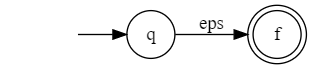
\includegraphics[width=2in, keepaspectratio]{tompson_rule1.png} % the Rule1 diagram placeholder

        Символ $a$ входного алфавита преобразуется в

        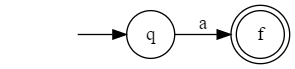
\includegraphics[width=2in, keepaspectratio]{tompson_rule2.png} % the Rule2 diagram placeholder
    }
    \only<2> {
        Выражение объединения $s\alter t$ преобразуется в

        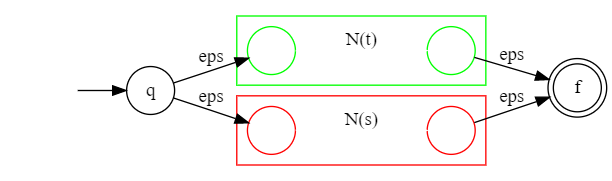
\includegraphics[width=4in, keepaspectratio]{tompson_rule3.png} % the Rule3 diagram placeholder

        Состояние $q$ переходит через $\empt$ либо в начальное состояние $N(s)$, либо $N(t)$. Их конечные состояния становятся промежуточными состояниями всего НКА и сливаются через два $\empt$-перехода в конечное состояние НКА.
    }
    \only<3> {
        Выражение конкатенации $st$ преобразуется в

        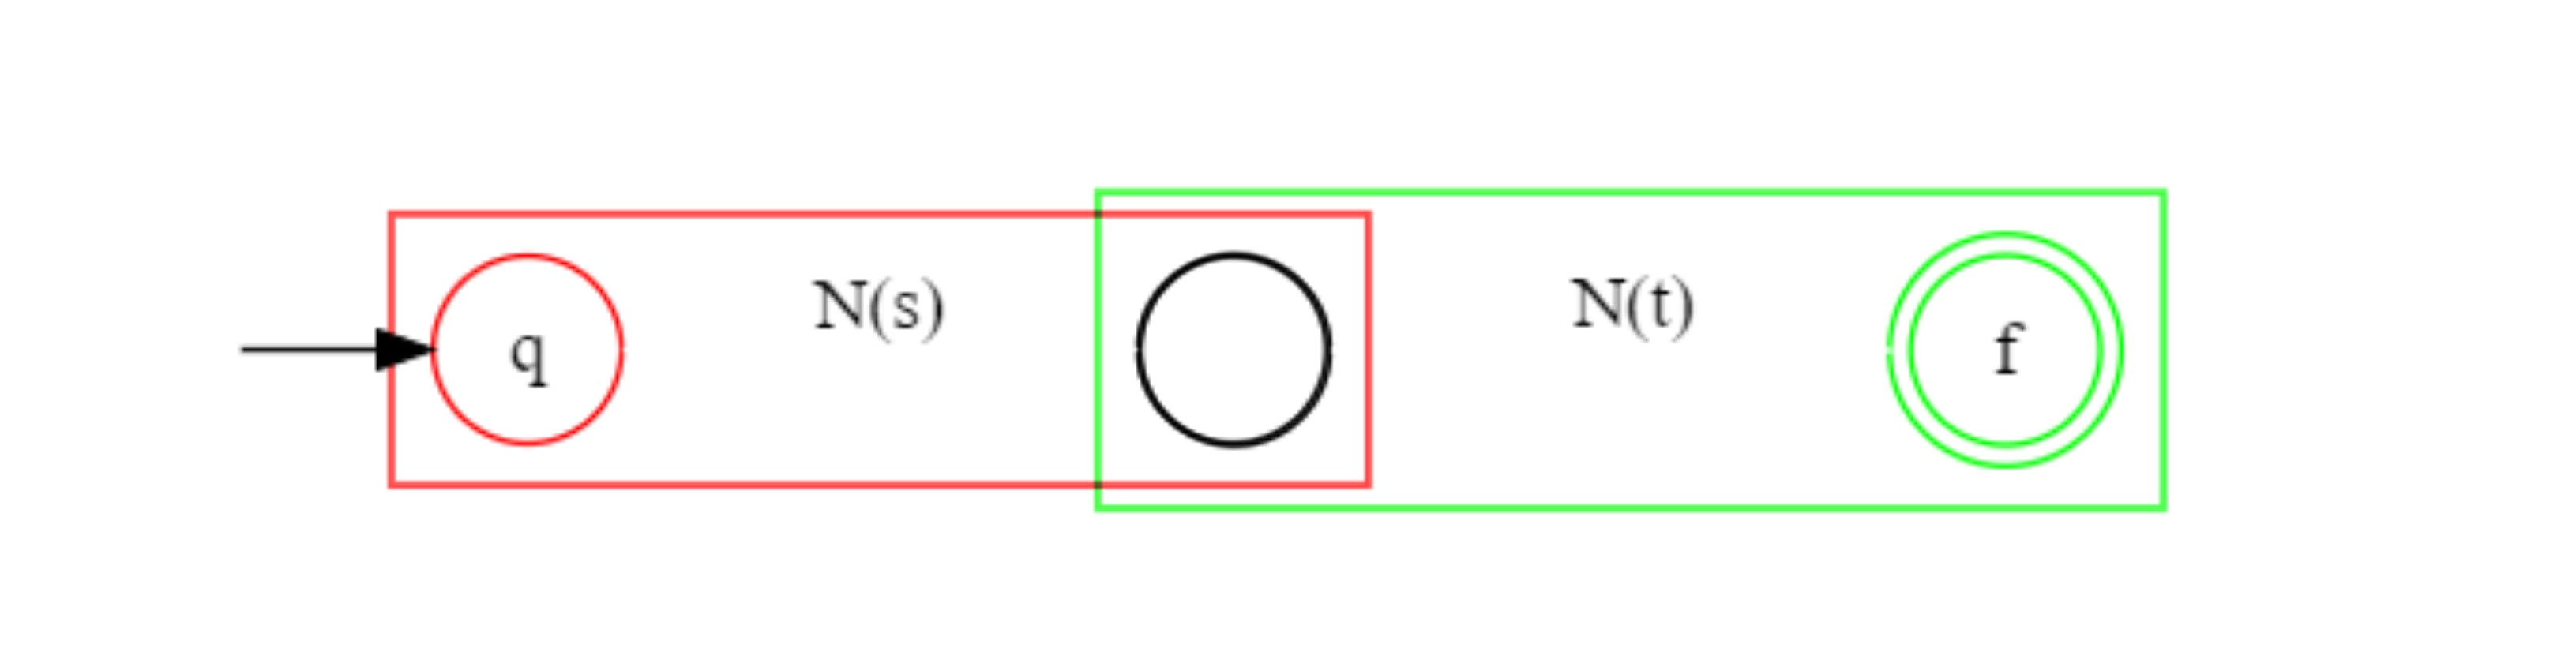
\includegraphics[width=4in, keepaspectratio]{tompson_rule4.png} % the Rule4 diagram placeholder

        Начальное состояние $N(s)$ является начальным состоянием всего НКА. Конечное состояние $N(s)$ становится начальным состоянием $N(t)$. Конечное состояние $N(t)$ является конечным состоянием всего НКА.
    }
    \only<4> {
        Выражение Клини Стар $s\star$ преобразуется в

        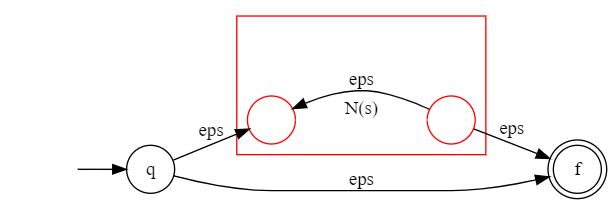
\includegraphics[width=4in, keepaspectratio]{tompson_rule5.png} % the Rule5 diagram placeholder

        $\empt$-переход соединяет начальное и конечное состояние НКА с промежуточным НКА $N(s)$. Другой $\empt$-переход от внутреннего конечного к внутреннему начальному состоянию $N(s)$ допускает повторение выражения $s$ в соответствии с оператором $\star$.

        Заключенное в скобки выражение (выражения) преобразуется в само $N(s)$.
    }
\end{frame}% descriptive documentation

\begin{frame}{Пример автомата Томпсона}
    Исходное регулярное выражение:
    \[(\regexpstr{a}\alter \regexpstr{b})\star\regexpstr{b}\] % the initial regexp placeholder displaystyle

    Автомат Томпсона:

    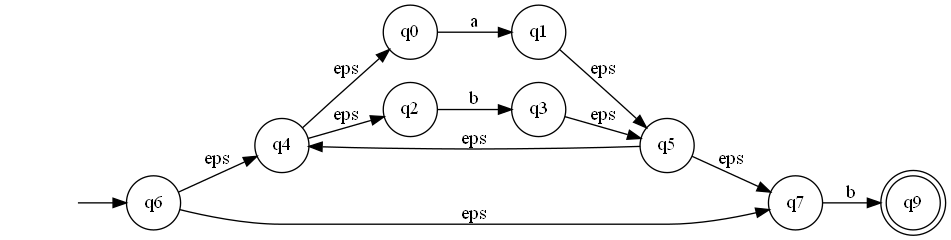
\includegraphics[width=4in, keepaspectratio]{tompson2.png} % the Tompson diagram placeholder
\end{frame}

% overall documentation : section 
\section{Обсуждение}
\begin{frame}{Cвойства автомата Томпсона}
    \begin{itemize}
        \item Единственное начальное состояние
        \item Единственное конечное состояние
        \item Не больше двух переходов из каждого состояния
    \end{itemize}
\end{frame}
\end{document}
